% CREATED BY DAVID FRISK, 2015
\chapter{Results}
%%%%%%

\section{Visualization from phase I}
The subsystem Visibility Control SPA has 18 LCs and 179 ports. The lines seen in the diagram~\ref{}. shows the association between the ports on each LCs. The LC which do not have ports nor connection are the ones which misses the connection the rest of the LCs. These are LC2, LC4, LC16 and LC16. Some of the LCs seems to be having a lot of ports and overlapping of data in it, these are LC3, LC6, LC10, LC17, LC18. The reason to that it is because the ports of these LCs connect to many other ports.  
\todo{[to be filled in]}


\begin{figure}[H]
\centering
\captionsetup{justification=centering}
\vspace{0cm}% Adjust vertical spacing here
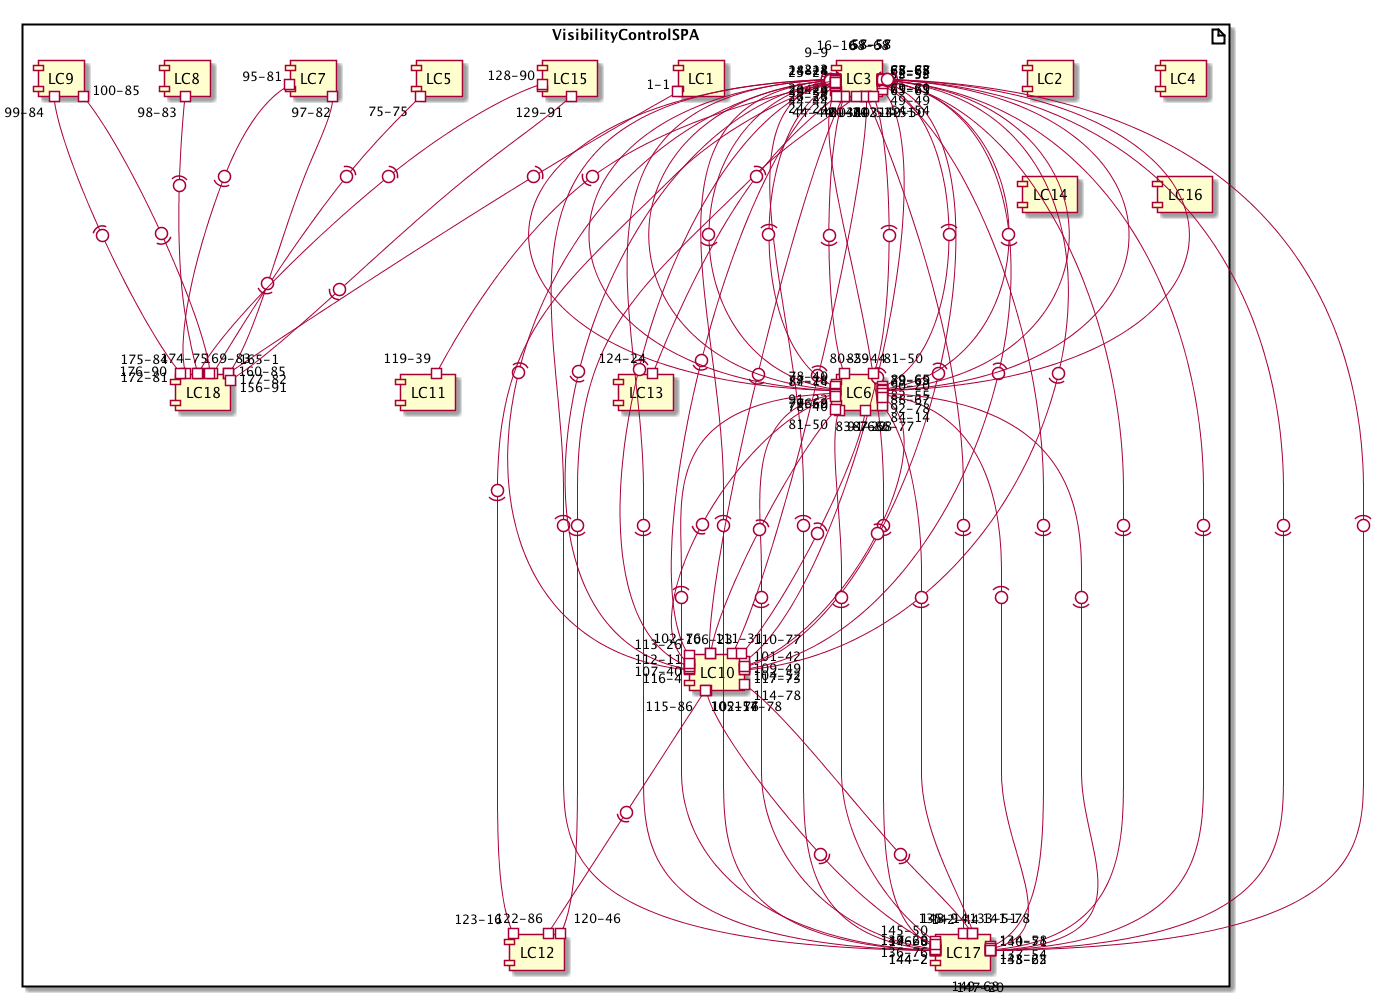
\includegraphics[width=1\linewidth]{figure/results/visualization_1.png}
\caption{Visualization}
\end{figure}

\todo{[to be filled in]}


\section{Visualization from phase II}
\todo{[to be filled in]}


\section{Evaluation of the visualization}
\todo{[to be filled in]}
